\documentclass{article}
\usepackage[russian]{babel}
\usepackage[utf8]{inputenc}
\usepackage{amsthm}
\usepackage{amsmath}
\usepackage{amsfonts}
\usepackage{mathtools}
\usepackage{graphicx}
\usepackage{mathrsfs}

\newtheorem{lemma}{Лемма}
\newtheorem{definition}{Определение}
\newtheorem{theorem}{Теорема}

\begin{document}
	\begin{definition}
		Циклической перестановкой из $k$ элементов с шагом $s$ будем называть такую циклическую перестановку, в которой элемент с номером $i$ переходит в элемент с номером $i+s \hspace{5pt} (\mod k)$. 
	\end{definition}

	Далее будем считать, что элементы перестановки длины $k$ - это числа от $0$ до $k-1$.
	
	\begin{lemma}
		Существуют такие перестановки $x$ и $y$ из $S_k$, что $xy$ - циклическая перестановка с шагом -1, а $yx$ - циклическая перестановка с шагом 1.
	\end{lemma}
	\begin{proof}
		Рассмотрим перестановку $x$: $i \rightarrow -i (\mod k)$ и $y$: $i \rightarrow -i+1 (\mod k)$.
		$$
		x = 
		\begin{pmatrix}
		0&1&2&3&...&k-3&k-2&k-1\\
		0&k-1&k-2&k-3&...&3&2&1
		\end{pmatrix}
		$$
		
		$$
		y = 
		\begin{pmatrix}
		0&1&2&3&...&k-3&k-2&k-1\\
		1&0&k-1&k-2&...&4&3&2
		\end{pmatrix}
		$$
		
		Тогда 
		
		$xy$: $i \xrightarrow y (-i+1) \xrightarrow x (-(-i+1)) == i-1$,
		
		$yx$: $i \xrightarrow x (-i) \xrightarrow y (-(-i)+1) == i+1$
		
	\end{proof}
	
	\begin{lemma}
		Пусть $(xy)^a(yx)^b(xy)^c$ = $(yx)^c(xy)^b(yx)^a$ - тождество в $S_k$, где $k$ - нечетное. Тогда $a - b + c \equiv 0 \hspace{5pt} (\mod k)$.
	\end{lemma}
	\begin{proof}
		Зафиксируем перестановки $xy$ и $yx$ из Леммы 1.
		Рассмотрим перестановочный автомат, в котором переход по символам осуществляется соответствующими перестановками $x$ и $y$. Тогда, чтобы $(xy)^a(yx)^b(xy)^c$ = $(yx)^c(xy)^b(yx)^a$ было тождеством для такого автомата, требуется, чтобы автомат закончил читать обе части равенства в одном состоянии, то есть	
		\begin{equation}
			(-a) + b + (-c) \equiv c + (-b) + a \hspace{5pt} (\mod k)
		\end{equation}
		что эквивалентно 
		\begin{equation}
		2(a - b + c) \equiv 0 \hspace{5pt} (\mod k)
		\end{equation}
		Из того, что $k$ нечетно, следует 
		$$
			(a - b + c) \equiv 0 \hspace{5pt} (\mod k)
		$$.
	\end{proof}

	\begin{lemma}
		Существуют такие перестановки $x$ и $y$, что $xy$ - циклическая перестановка с шагом 1, а $yx$ - циклическая перестановка с шагом 1, в которой поменяли местами элементы $a$ и $b$.
	\end{lemma}
	\begin{proof}
		Без ограничения общности $a < b$.
		Требуется, чтобы $xy$ = (0, 1, 2, ..., $k-1$), а $yx$ = (0, 1, ..., $a-1$, $b$, $a+1$, ..., $b-1$, $a$, $b+1$, ..., $k-1$).
		
		Пусть $y$ переводит $a-1$ в $b$, $b-1$ в $a$, а любой другой элемент в следующий, то есть
		$$
		y = 
		\begin{pmatrix}
			0&...&a-2&a-1&a&...&b-2&b-1&b&...\\
			1&...&a-1&b&a+1&...&b-1&a&b+1&...
		\end{pmatrix}
		$$
		а $x$ переводит $a$ в $b$ и наоборот, а остальные элементы оставляет на месте:
		
		$$
		x = 
		\begin{pmatrix}
			0&...&a-1&a&a+1&...&b-1&b&b+1&...\\
			0&...&a-1&b&a+1&...&b-1&a&b+1&...
		\end{pmatrix}
		$$
		Откуда получим 
		$$
		xy = 
		\begin{pmatrix}
			0&...&a-2&a-1&a&...&b-2&b-1&b&...\\
			1&...&a-1&a&a+1&...&b-1&b&b+1&...
		\end{pmatrix}
		$$
		$$
		yx = 
		\begin{pmatrix}
			0&...&a-2&a-1&a&...&b-2&b-1&b&...\\
			1&...&a-1&b&b+1&...&b-1&a&a+1&...
		\end{pmatrix}
		$$
		Что и требовалось найти.
	\end{proof}

	\begin{theorem}
		 Пусть $(xy)^a(yx)^b(xy)^c$ = $(yx)^c(xy)^b(yx)^a$ - тождество в $S_k$, $k$ - нечетное число, $k > 3$. Тогда выполняется хотя бы одно из следующих правил:
		 \begin{equation*}
		 k|a \hspace{10pt} \text{и} \hspace{10pt} k|(b-c)
		 \end{equation*}
		 \begin{equation*}
		 k|c \hspace{10pt} \text{и} \hspace{10pt} k|(b-a)
		 \end{equation*}
		 \begin{equation*}
		 k|b \hspace{10pt} \text{и} \hspace{10pt} k|(a+c)
		 \end{equation*}
	\end{theorem}
	\begin{proof}
		От противного. Допустим, ни одно из перечисленных правил не выполняется, то есть ни одно из чисел $a$, $b$, $c$ не делится на $k$. Тогда с учетом Леммы 2 на $k$ не делятся и числа $b-a$, $b-c$, $a+c$. Тогда найдутся автоматы, различающие строки справа и слева от знака равенства. Рассмотрим несколько случаев.
		
		В представленных ниже автоматах удобно будет оперировать не только значением состояния в автомате, но и номером этого состояния в цикле.
		Существование рассматриваемых автоматов доказано Леммой 3.
		
		\begin{enumerate}
			\item $a+b \not \equiv 0 (\mod k)$
			
			Рассмотрим перестановочный автомат $\mathscr{A}$ такой, что $xy$ действует на него как циклическая перестановка из $k$ элементов с шагом 1, а $yx$ - как циклическая перестановка из $k$ элементов с шагом 1, в которой поменяли местами элементы $a+b$ и $b$ (см. Рис. \ref{cycle_a+b_b}). $a+b$ и $b$ не равны 0 по модулю $k$, $a+b \ne b$, так как $a$ не делится на $k$. Начальное состояние 0.
			
			\begin{figure}
				\centering{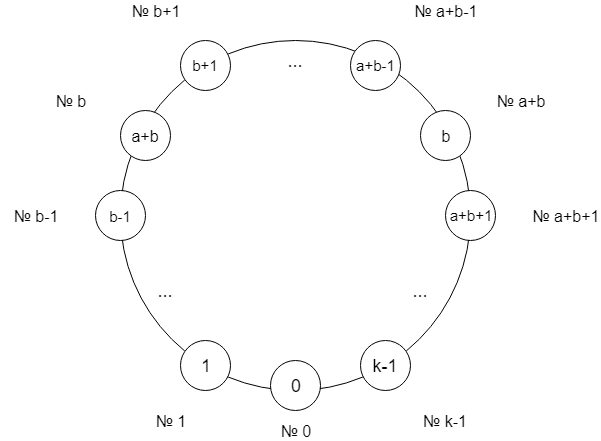
\includegraphics[scale=0.5]{images/cycle_a+b_b}}
				\caption{Перестановка $yx$ автомата $\mathscr{A}$}
				\label{cycle_a+b_b}
			\end{figure}
		
			Покажем, что такой автомат различит слова $(xy)^a(yx)^b(xy)^c$ и\\ $(yx)^c(xy)^b(yx)^a$.
			
			Автомат $\mathscr{A}$ закончит читать слово $(xy)^a(yx)^b(xy)^c$ в состоянии $b+c$ (см. Рис \ref{process1_cycle_a+b_b}).
			
			\begin{figure}
				\centering{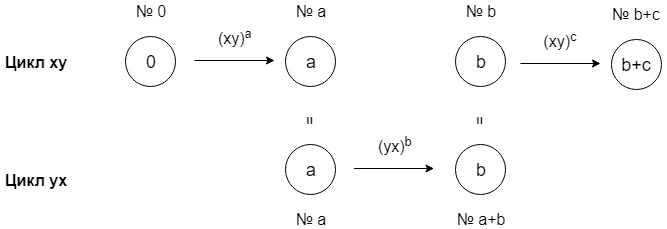
\includegraphics[scale=0.5]{images/process1_a+b_b}}
				\caption{Чтение автоматом $\mathscr{A}$ слова $(xy)^a(yx)^b(xy)^c$}
				\label{process1_cycle_a+b_b}
			\end{figure}
			
			Корректность переходов при чтении $(xy)^a(yx)^b(xy)^c$:
			\begin{itemize}
				\item $0 \xrightarrow{(xy)^a} a$
				\begin{itemize}
					\item $a \not \equiv a+b$, так как $b \not \equiv 0 \mod k$
					\item $a \not \equiv b$, так как $b-a \not \equiv 0 \mod k$
				\end{itemize}
				\item $a \xrightarrow{(yx)^b} b$
				\begin{itemize}
					\item Из состояния с номером $a$ делаем $b$ шагов, оказываемся в состоянии с номером $a+b$, которым в данном цикле является $b$, т.к. мы так задали автомат.
				\end{itemize}
			\end{itemize}
			
			Теперь покажем, что $\mathscr{A}$ не закончит читать слово $(yx)^c(xy)^b(yx)^a$ в состоянии $b+c$ (см. Рис \ref{process2_cycle_a+b_b}).
			
			\begin{figure}
				\centering{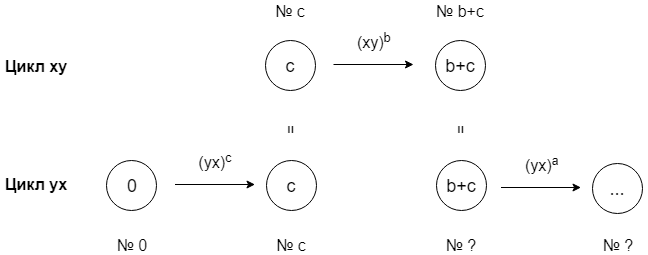
\includegraphics[scale=0.5]{images/process2_a+b_b}}
				\caption{Чтение автоматом $\mathscr{A}$ слова $(yx)^c(xy)^b(yx)^a$}
				\label{process2_cycle_a+b_b}
			\end{figure}
		
			Корректность переходов при чтении $(yx)^c(xy)^b(yx)^a$:
			\begin{itemize}
				\item $0 \xrightarrow{(yx)^c} c$
				\begin{itemize}
					\item $c \not \equiv a+b$. 
					
					От противного. Пусть $c \equiv a+b (\mod k)$. Тогда $a+b-c \equiv 0 (\mod k)$ и $a-b+c \equiv 0 (\mod k)$ по Лемме 2. Сложив оба равенства получим $2a \equiv 0 (\mod k)$. Но $k$ нечетно, поэтому $a \equiv 0 (\mod k)$. Противоречие.
					\item $c \not \equiv b$, так как $b-c \not \equiv 0 \mod k$
				\end{itemize}
				\item Переход $c \xrightarrow{(xy)^b} b+c$ осуществляется в обычном цикле без ловушки. Последний переход выполняется из состояния $b+c$. Поскольку $a \not \equiv 0 (\mod k)$, переход по $(yx)^a$ не вернет автомат обратно в состояние $b+c$. 
			\end{itemize}
		
			\item $a+b \equiv 0 (\mod k)$ и $a \not \equiv c (\mod k)$
			
			Из того, что $a+b \equiv 0 (\mod k)$, следует $a+c \not \equiv 0 (\mod k)$ (иначе, выразив $a$ из первого утверждения и подставив его во второе, получили бы $c-b \equiv 0 (\mod k)$, что противоречит нашему предположению).
			
			Рассмотрим перестановочный автомат $\mathscr{B}$, в котором  перестановка $xy$ - это циклическая перестановка из $k$ элементов с шагом 1, а $yx$ - циклическая перестановка из $k$ элементов с шагом 1, в которой состояния $a$ и $a+c$ поменяли местами (см. Рис. \ref{cycle_a+c_a}). Начальное состояние 0.
			
			\begin{figure}
				\centering{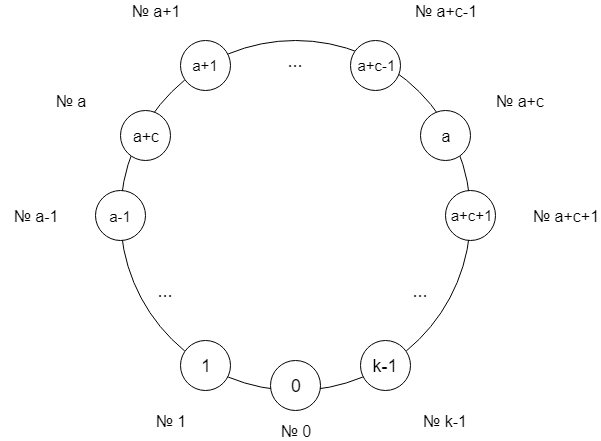
\includegraphics[scale=0.5]{images/cycle_a+c_a}}
				\caption{Перестановка $yx$ автомата $\mathscr{B}$}
				\label{cycle_a+c_a}
			\end{figure}
		
			Покажем, что такой автомат различит слова $(xy)^a(yx)^b(xy)^c$ и\\ $(yx)^c(xy)^b(yx)^a$.
			
			\begin{figure}
				\centering{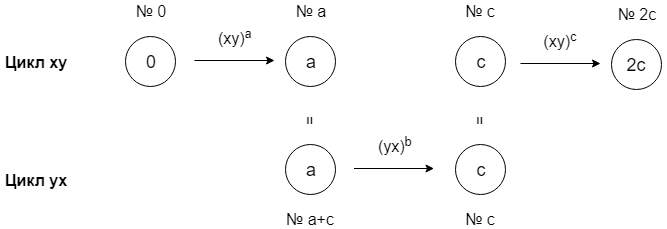
\includegraphics[scale=0.5]{images/process1_a+c_a}}
				\caption{Чтение автоматом $\mathscr{B}$ слова $(xy)^a(yx)^b(xy)^c$}
				\label{process1_a+c_a}
			\end{figure}
			
			Автомат $\mathscr{B}$ закончит читать слово $(xy)^a(yx)^b(xy)^c$ в состоянии $2c$ (см. Рис. \ref{process1_a+c_a}).
			
			Корректность переходов:
			\begin{itemize}
				\item $a \xrightarrow{(yx)^b} c$
				\begin{itemize}
					\item $a+c+b \equiv c (\mod k)$ потому что $a+b \equiv 0 (\mod k)$
					\item $c \not \equiv a (\mod k)$ по выбранному ограничению
					\item $c \not \equiv a+c (\mod k)$ потому что $a \not \equiv 0 (\mod k)$
				\end{itemize}
			\end{itemize}
		
			Теперь покажем, что автомат $\mathscr{B}$ закончит читать слово $(yx)^c(xy)^b(yx)^a$ в состоянии $c$, которое, очевидно, не совпадает с состоянием $2c$ (см. Рис. \ref{process2_a+c_a})
			
			\begin{figure}
				\centering{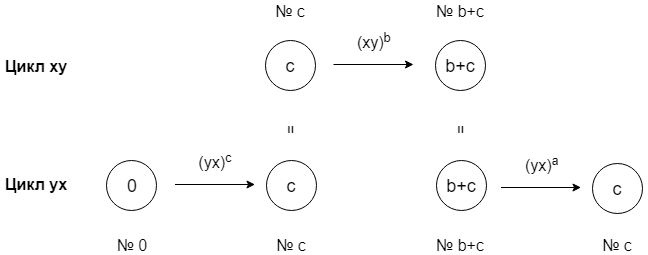
\includegraphics[scale=0.5]{images/process2_a+c_a}}
				\caption{Чтение автоматом $\mathscr{B}$ слова $(yx)^c(xy)^b(yx)^a$}
				\label{process2_a+c_a}
			\end{figure}
		
			Корректность переходов:
			\begin{itemize}
				\item $0 \xrightarrow{(yx)^c} c$
				\begin{itemize}
					\item $c \not \equiv a (\mod k)$ по выбранному ограничению
					\item $c \not \equiv a+c (\mod k)$ потому что $a \not \equiv 0 (\mod k)$, поэтому не попадаем в "ловушку"
				\end{itemize}
			
				\item $c \xrightarrow{(xy)^b} b+c$
				\begin{itemize}
					\item $b+c \not \equiv a+c (\mod k)$, т.к. $b-a \not \equiv 0 (\mod k)$ по предположению
					\item $b+c \not \equiv a (\mod k)$
					
					От противного. Пусть $b+c \equiv a (\mod k)$, тогда $b+c-a \equiv 0 (\mod k)$. Сложим с $a-b+c \equiv 0 (\mod k)$, получим $2c \equiv 0 (\mod k)$. Поскольку $k$ нечетное, имеем $c \equiv 0 (mod k)$ и получаем противоречие.
				\end{itemize}
			
				\item $b+c \xrightarrow{(yx)^a} c$
				\begin{itemize}
					\item $b+c+a \equiv c (\mod k)$, т.к. $a+b \equiv 0 (\mod k)$ по ограничению. А $c$ не попадает в "ловушку".
				\end{itemize}
			\end{itemize}
		
			\item $a+b \equiv 0 (\mod k)$ и $a \equiv c (\mod k)$
			
			Из того, что $a+b \equiv 0 (\mod k)$ следует, что $b \equiv -a (\mod k)$.
			
			Из того, что $a-b+c \equiv 0 (\mod k)$ и $a \equiv c (\mod k)$ следует, что $b \equiv 2a (\mod k)$. 
			
			То есть $2a \equiv -a$ или $3a \equiv 0 (\mod k)$.
			
			Если $k$ не делится на 3, получаем $a \equiv 0 (\mod k)$, что противоречит предположению.
			
			Пусть $k = 3m$, $m \in \mathbb{N}$. Тогда $a \equiv c \equiv m (\mod k)$, $b \equiv 2m (\mod k)$.
			
			\begin{figure}
				\centering{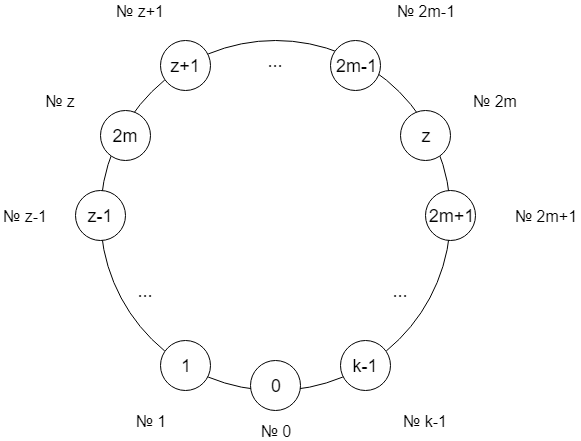
\includegraphics[scale=0.5]{images/cycle_2m_z}}
				\caption{Цикл $yx$ автомата $\mathscr{C}$}
				\label{cycle_2m_z}
			\end{figure}
			
			Рассмотрим перестановочный автомат $\mathscr{C}$ с начальным состоянием $m$, такой, что $xy$ - циклическая перестановка из $k$ элементов с шагом 1, а $yx$ - циклическая перестановка из $k$ элементов с шагом 1, в которой поменяли местами состояния $2m$ и $z$, где $z \not \equiv 0 (\mod k)$, $z \not \equiv m (\mod k)$ и $z \not \equiv 2m (\mod k)$ (см. Рис. \ref{cycle_2m_z}). Такое $z$ существует, если $k > 3$.
			
			Покажем, что автомат $\mathscr{C}$ закончит читать слова $(xy)^a(yx)^b(xy)^c$ и $(yx)^c(xy)^b(yx)^a$ в разных состояниях.
			
			При чтении слова $(xy)^a(yx)^b(xy)^c$ автомат $\mathscr{C}$ остановится в состоянии $z$ (см. Рис. \ref{process1_2m_z})
			
			\begin{figure}
				\centering{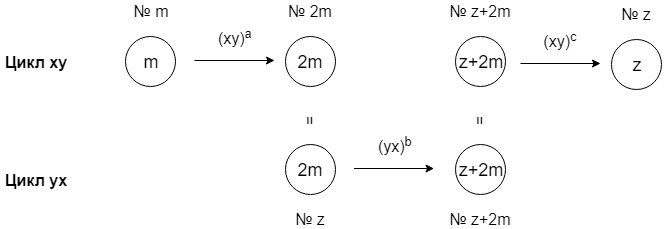
\includegraphics[scale=0.5]{images/process1_2m_z}}
				\caption{Чтение слова $(xy)^a(yx)^b(xy)^c$ автоматом $\mathscr{C}$}
				\label{process1_2m_z}
			\end{figure}
		
			Корректность переходов:
			\begin{itemize}
				\item $2m \xrightarrow{(yx)^b} 2m+z$
				\begin{itemize}
					\item $2m+z \not \equiv x (\mod k)$, т.к. $2m < k$, а значит $2m \not \equiv 0 (\mod k)$
					\item $2m+z \not \equiv 2m (\mod k)$ по выбору $z$\\
				\end{itemize}
			
				\item $z+2m \xrightarrow{(xy)^c} z$
				\begin{itemize}
					\item $z+2m+m \equiv z+k \equiv z (\mod k)$
				\end{itemize}
			\end{itemize}
		
			При чтении слова $(yx)^c(xy)^b(yx)^a$ автомат $\mathscr{C}$ остановится в состоянии $2m$, которое не совпадает с $z$ (см. Рис. \ref{process2_2m_z})
			
			\begin{figure}
				\centering{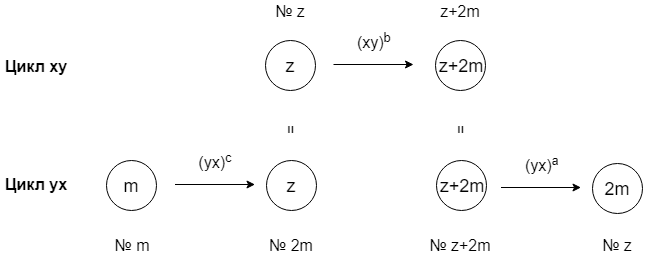
\includegraphics[scale=0.5]{images/process2_2m_z}}
				\caption{Чтение слова $(yx)^c(xy)^b(yx)^a$ автоматом $\mathscr{C}$}
				\label{process2_2m_z}
			\end{figure}
		
			Корректность переходов:
			\begin{itemize}
				\item $z+2m \xrightarrow{(yx)^c} 2m$
				\begin{itemize}
					\item $z+2m+m \equiv z+k \equiv z (\mod k)$
					\item Под номером $z$ в цикле $yx$ находится состояние $2m$ по выбору автомата
				\end{itemize}
			\end{itemize}
		\end{enumerate}
	
		В итоге, три рассмотренных случая покрывают всевохможные варианты $a$, $b$ и $c$, и ни один не привел к успеху. Значит, наше предположение о невыполнении правил было ложным.
	\end{proof}
\end{document}